\documentclass[12pt,b5paper]{ltjsarticle}

%\usepackage[margin=15truemm, top=5truemm, bottom=5truemm]{geometry}
\usepackage[margin=15truemm]{geometry}

\usepackage{amsmath,amssymb}
%\pagestyle{headings}
\pagestyle{empty}


\usepackage{graphicx}
\usepackage{wrapfig}


%\usepackage{listings,url}
\renewcommand{\theenumi}{(\arabic{enumi})}

\begin{document}

\begin{wrapfigure}[7]{R}{130pt}
 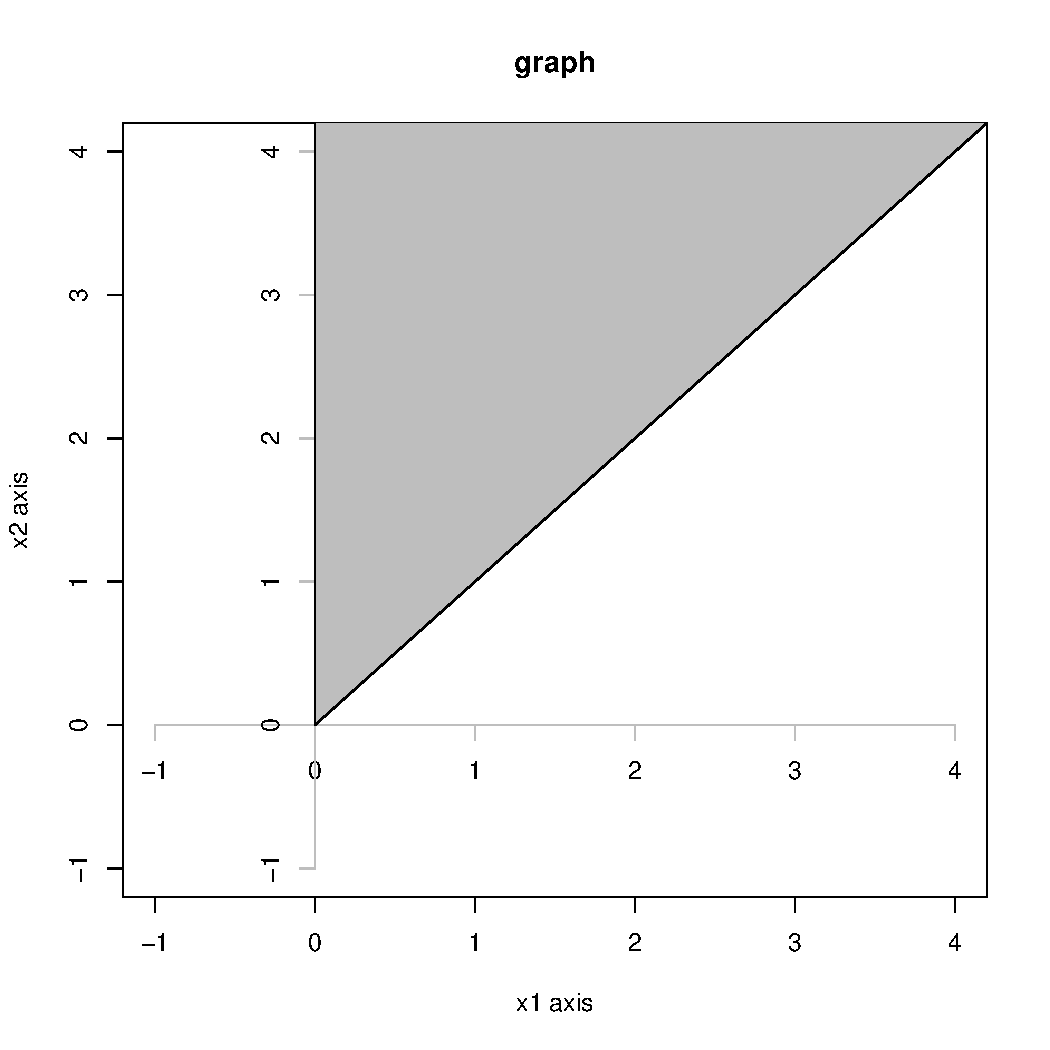
\includegraphics[scale=0.3]{graph_R.pdf}
\end{wrapfigure}



$g(x_1, x_2) = \exp(-x_1 -2x_2)$を

$D=\{ (x_1, x_2) \in \mathbb{R}^2 | x_2 \geq x_1 \geq 0 \}$
上で積分せよ。

\hrulefill


領域$D$での積分は$x_1$が区間$[0, x_2]$範囲で積分することになり、
$x_2$は$0$以上の範囲で積分をする。(右の図)
この為、次のような式に変形できる。

\begin{align}
 \iint_{D} \exp(-x_1 -2x_2) d{x_1} d{x_2}
  &= \int_0^{\infty} \int_0^{x_2} \exp(-x_1 -2x_2) d{x_1} d{x_2}\\
  &= \lim_{n \rightarrow \infty}\int_0^{n} \int_0^{x_2} \exp(-x_1 -2x_2) d{x_1} d{x_2}\label{020542_28Mar22}
\end{align}

内側の$x_1$における積分は次のように求められる。
\begin{align}
  \int_0^{x_2} \exp(-x_1 -2x_2) d{x_1}
 &= \left[ -\exp(-x_1 -2x_2) \right]_{x_1=0}^{x_1=x_2}\\
 &= -\exp(-x_2 -2x_2) +\exp(-0 -2x_2)\\
 &= -\exp( -3x_2) +\exp( -2x_2)
\end{align}

これを
(\ref{020542_28Mar22})の式に
代入する。

\begin{align}
 & \lim_{n \rightarrow \infty}\int_0^{n} \int_0^{x_2} \exp(-x_1 -2x_2) d{x_1} d{x_2}\\
 =& \lim_{n \rightarrow \infty}\int_0^{n} (-\exp( -3x_2) +\exp( -2x_2))  d{x_2}\\
 =& \lim_{n \rightarrow \infty} \left[ \frac{1}{3} \exp( -3x_2) -\frac{1}{2}\exp( -2x_2) \right]_{x_2=0}^{x_2=n}\\
 =& \lim_{n \rightarrow \infty} \left( \frac{1}{3} \exp( -3n) -\frac{1}{2}\exp( -2n) - \frac{1}{3} +\frac{1}{2}\right)\\
 =&  \frac{1}{3}\times 0 -\frac{1}{2}\times 0 - \frac{1}{3} +\frac{1}{2}
 = \frac{1}{6}
\end{align}

\begin{equation}
  \iint_{D} \exp(-x_1 -2x_2) d{x_1} d{x_2}
   = \frac{1}{6}
\end{equation}

\end{document}
